\documentclass[a4paper,12pt,twoside]{article}
\usepackage[utf8]{inputenc}
\usepackage[T1]{polski}
\usepackage{helvet}
\usepackage{graphicx}
\usepackage[export]{adjustbox}
\usepackage{color}
\usepackage{listings}
\usepackage{leading}
\usepackage{lipsum}
\usepackage{float}
\usepackage{diagbox}
\usepackage{amsfonts}
\usepackage{makecell}
\usepackage{url}
\usepackage[none]{hyphenat} 
\usepackage{hyperref}
\usepackage{chngpage}
\usepackage{graphicx}% http://ctan.org/pkg/graphicx
\usepackage{array}% http://ctan.org/pkg/array
\hypersetup{
    colorlinks,
    citecolor=black,
    filecolor=black,
    linkcolor=black,
    urlcolor=black
}
\usepackage{tocloft}
\renewcommand\cftsecleader{\cftdotfill{\cftdotsep}}
\usepackage{fancyhdr}
\usepackage[top=2.5cm,bottom=2.5cm,inner=3.5cm,outer=2.5cm]{geometry}
\leading{20pt}

\tolerance=1
\emergencystretch=\maxdimen
\hyphenpenalty=10000
\hbadness=10000

\pagestyle{fancy}
\fancyhf{}
\fancyhead{}
\fancyhead[RO,LE]{\nouppercase{\leftmark}}
\fancyfoot[C]{\thepage}
\renewcommand{\headrulewidth}{0.4pt}
\newcommand\tab[1][1cm]{\hspace*{#1}}

\begin{document}
% ===============  STRONA TYTULOWA PRACY MAGISTERSKIEJKIEJ ==============
\thispagestyle{empty}
%% ------------------------ NAGLOWEK STRONY ------------------------------

\includegraphics[height=37.5mm]{dudel.jpg}\\
\rule{30mm}{0pt}
{\large \textsf{Wydział Fizyki i Informatyki Stosowanej}}\\
\rule{\textwidth}{3pt}\\
\rule[2ex]
{\textwidth}{1pt}\\

\vspace{1ex}

\begin{center}
{\LARGE \bf \textsf{Praca magisterska}}\\

\vspace{10ex}

% --------------------------- IMIE I NAZWISKO ----------------------------
{\bf \Large \textsf{Kamil Madej}}\\
\vspace{3ex}
{\sf\small kierunek studiów:} {\bf\small \textsf{Informatyka Stosowana}}\\
\vspace{1.5ex}
{\sf\small specjalność:} {\bf\small \textsf{Grafika Komputerowa i Przetwarzanie Obrazów}}\\
\vspace{10ex}
%% ------------------------ TYTUL PRACY ----------------------------------
{\bf \huge \textsf{Sposoby zwiększania bezpieczeństwa systemu informatycznego przy pomocy aplikacji do zarządzania zasobami systemów informatycznych}}\\
\vspace{10ex}
%% ------------------------ OPIEKUN PRACY --------------------------------
{\Large Opiekun: \bf \textsf{dr inż. Antoni Dydejczyk}}\\
\vspace{10ex}
{\large \bf \textsf{Kraków, czerwiec 2018}}
\end{center}
%% ===============  STRONA TYTULOWA PRACY MAGISTERSKIEJKIEJ ==============

\newpage
%% ============= TYL STRONY TYTULOWEJ PRACY MAGISTERSKIEJKIEJ ============
{\sf Oświadczam, świadomy odpowiedzialności karnej za poświadczenie nieprawdy, że niniejszą pracę dyplomową wykonałem osobiście i samodzielnie i  nie korzystałem ze źródeł innych niż wymienione w pracy.}
\vspace{14ex}
\begin{flushright}
\begin{tabular}{lr}
~~~~~~~~~~~~~~~~~~~~~~~~~~~~~~~~~~~~~~~~~~~~~~~~~~ &
................................................................. \\
~ & {\sf (czytelny podpis)}\\
\end{tabular}
\end{flushright}

\newpage
%% ============================== DEDYKACJA =============================
\mbox{}
\vfill{%
\begin{flushright}
    TODO
\end{flushright}
}

\mbox{}

\newpage
%% ===============  TEMATYKA PRACY MAGISTERSKIEJKIEJ ===================
\rightline{Kraków, czerwiec 2018}
\begin{center}
{\bf Tematyka pracy magisterskiej i praktyki dyplomowej
Kamila Madeja,
studenta V roku studiów kierunku informatyka stosowana, specjalności grafika komputerowa i przetwarzanie obrazów}\\
\end{center}

Temat pracy magisterskiej:
{\bf Sposoby zwiększania bezpieczeństwa systemu informatycznego przy pomocy aplikacji do zarządzania zasobami systemów informatycznych}\\

\begin{tabular}{rl}

Opiekun pracy:                  & dr inż. Antoni Dydejczyk\\
Recenzenci pracy:               & dr inż. TODO\\
Miejsce praktyki dyplomowej:    & WFiIS AGH, Kraków\\
\end{tabular}
\vspace{3ex}
\begin{center}
{\bf Program pracy magisterskiej i praktyki dyplomowej}
\end{center}

\begin{enumerate}
\item Omówienie realizacji pracy magisterskiej z opiekunem oraz przedstawicielem firmy IBM.
\item Zebranie i opracowanie literatury dotyczącej tematu pracy.
\item Praktyka dyplomowa:
\begin{itemize}
\item Zapoznanie się z ideą Software Asset Management
\item Zapoznanie się z tematyką podatności systemów informatycznych
\item Analiza danych wejściowych
\end{itemize}
\item Opracowanie algorytmu umożliwiającego wykrywanie podatności w systemie
\item Przeprowadzenie testów, analiza wyników
\item Porównanie otrzymanych wyników z próbami przeprowadzonymi przez IBM
\item Analiza wyników, ich omówienie i zatwierdzenie przez opiekuna
\item Opracowanie redakcyjne pracy
\end{enumerate}

\noindent
Termin oddania w dziekanacie: TODO czerwca 2018\\[1cm]

\begin{center}
\begin{tabular}{lcr}
.......................................................... & ~~~ &
.......................................................... \\
(podpis kierownika katedry) & & (podpis opiekuna) \\
\end{tabular}
\end{center}

\newpage
%% =========================  RECENZJE ==================================
\thispagestyle{empty}
\mbox{}

\null\newpage
Merytoryczna ocena pracy przez opiekuna: TODO

\newpage
\thispagestyle{empty}
\mbox{}

\null\newpage
Merytoryczna ocena pracy przez recenzenta: TODO

\newpage
%% =========================  SPIS TRESCI ================================
\thispagestyle{empty}
\mbox{}
\null\newpage
\tableofcontents


\newpage
%% ============================ WSTEP ====================================
\section*{Wstęp}
\addcontentsline{toc}{section}{Wstęp}
\markboth{Wstęp}{}
\paragraph{}
    Software Asset Management jest pojęciem ściśle związanym z dynamicznie rozwijającym się rynkiem oprogramowania. Pojawiające się różne rodzaje licencji określające sposób, w jaki można korzystać z poszczególnych rozwiązań, stworzyły przestrzeń dla firm takich, jak IBM, na stworzenie aplikacji ułatwiającej zarządzanie licencjami w systemach informatycznych przedsiębiorstw. W dzisiejszych realiach poważne przedsiębiorstwa muszą działać transparentnie, nie mogą sobie bowiem pozwolić na oskarżenia o nadużywanie lub nieprzestrzeganie wymogów licencyjnych. Wiąże się to nie tylko z kosztami ponoszonymi wskutek naliczanych kar, ale też ze stratami wizerunkowymi.

    \paragraph{}
    Każdego dnia pojawiają się nowe podatności i zagrożenia, na jakie wystawione są systemy informatyczne. Twórcom oprogramowania zależy, aby ich produkt był jak najbardziej na nie odporny. Wymusza to publikowanie nowych wersji oprogramowania, w którym poprawiono błędy i załatano luki umożliwiające niepożądane działanie systemu.      

    \paragraph{}
    Niniejsza praca jest próbą połączenia powyższych pojęć w jednym narzędziu. Wykorzystując informacje gromadzone w aplikacji IBM Big Fix Inventory, można informować użytkownika o tym, że w jego systemie informatycznym zainstalowane jest oprogramowanie, w którym wykryta została podatność. Właściciel systemu na podstawie informacji o rodzaju podatności i o stopniu zagrożenia z nią związanego, może zdecydować jakie akcje należy podjąć, by zapewnić stabilność i bezpieczeństwo systemu.

    \paragraph{}
    Algorytm opracowany w ramach pracy umożliwia wykrycie w systemie informatycznym wersji oprogramowania znajdujących się na liście obciążonych podatnościami, publikowanej przez amerykańską agencję NIST. Jego działanie polega na dopasowaniu informacji o oprogramowaniu zainstalowanym i używanym w systemie, zebranych przez IBM Big Fix Inventory, z informacjami zebranymi przez NIST.    
    
\paragraph{}



\newpage
%% =========================== CEL PRACY =================================
\section*{Cel pracy}
\addcontentsline{toc}{section}{Cel pracy}
\markboth{Cel pracy}{}
\paragraph{}
Niniejsza praca stanowi badanie możliwości wykorzystania różnych algorytmów porównania tekstu oraz ich połączeń w celu wykrywania oprogramowania, które może powodować podatność systemu informatycznego na zagrożenia. W ramach pracy zostaną wykonane następujące czynności:
\begin{itemize}
\item Analiza poszczególnych algorytmów pod kątem danych wejściowych. 
\item Na podstawie powyższej analizy zostanie opracowany algorytm pozwalający na połączenie dostępnych informacji o podatnościach występujących oprogramowaniu informatycznym oraz informacji o oprogramowaniu zainstalowanym w badanym systemie.
\item Implementacja algorytmu w języku Python
\item Przeprowadzenie testów skuteczności algorytmu
\item Analiza otrzymanych wyników
\end{itemize}
\paragraph{}
Podczas opracowywania algorytmu szczególna uwaga zwrócona będzie w kierunku skuteczności wykrycia zagrożonej wersji oprogramowania zainstalowanej w systemie informatycznym monitorowanym przez narzędzie IBM Big Fix Inventory. Efektem pracy będą przedstawione wnioski dotyczące efektywności poszczególnych algorytmów porównania tekstu oraz ich połączeń opracowanych w ramach pracy. Wnioski zostaną wyciągnięte na podstawie wyników testów poszczególnych rozwiązań.
\newpage
\thispagestyle{empty}
\mbox{}

\newpage
%% =========================== ROZDZIAL 1 ================================
\section{Software Asset Management}
\subsection{Wstęp}
\paragraph{}
Eksploracja danych zajmuje się analizą dużych zbiorów danych dotyczących różnych zjawisk. Mogą to być dane finansowe, wyniki obserwacji fizyczny czy dane pacjentów. Danych najczęściej jest zbyt dużo aby mógł je przeanalizować człowiek, dlatego też istnieje zapotrzebowanie na automatyczne algorytmy operujące na całym zbiorze danych. Zbiór zwykle przedstawiany jest w postaci macierzy której kolumnami są cechy opisujące zjawisko, a wiersze to kolejne obserwacje. Analizowane dane mogą mieć następujące typy:
\begin{itemize}
    \item Liczbowe - Numeryczny wynik jakiegoś pomiaru, na przykład wzrost, waga
    \item Kategoryczne - Wartość z ograniczonego zbioru, na przykład rozróżnienie kobiet i mężczyzn, czy grupy krwi
    \item Tekstowe - Bloki tekstu opisujące zjawisko, na przykład treść wiadomości e-mail 
\end{itemize}
\paragraph{}
\newpage
\thispagestyle{empty}
\mbox{}

\newpage
%% =========================== ROZDZIAL 2 ================================
\section{Reprezentacja danych}
\subsection{Common Vulnerabilities and Exposures}
\paragraph{}
Common Vulnerabilities and Exposures jest systemem zapewniającym publiczne, darmowe informacje na temat ekspozycji i podatności systemów informatycznych. Celem stworzenia CVE było utworzenie standardu, który ułatwiłby dzielenie się informacjami pomiędzy różnymi narzędziami i organizacjami zajmującymi się tematyką cyberbezpieczeństwa. Dzięki CVE możliwa stała się komunikacja pomiędzy tymi narzędziami, co pozwoliło na bardziej efektywną walkę z atakami na systemy informatyczne. 
\paragraph{}
W CVE podatność zdefiniowana jest jako słabość w logice obliczeniowej, znaleziona w oprogramowaniu lub komponentach sprzętowych, które, jeśli zostałyby odkryte, niekorzystnie wpłynęły by na poufność, integralność lub dostępność systemu. Naprawa podatności zwykle wymaga zmian w kodzie programu, czasem również zmian w specyfikacji. Ekspozycją (TODO przemyśleć tłumaczenie "exposure") jest błędna konfiguracja systemu lub błąd w oprogramowaniu, który daje dostęp do informacji i zdolności systemu, użytych później przez hakera jako wytrych\cite{cve_mitre_terms}.   
\paragraph{}
Lista Common Vulnerabilities and Exposures składa się CVE Entry, czyli wpisów CVE, które identyfikują poszczególne podatności. \newline Każdy wpis na liście CVE składa się z:
\begin{itemize}
\item CVE ID, który jest unikatowym identyfikatorem wpisu. Zapisany jest obecnie w formacie CVE-YYY-NNNN, gdzie YYYY jest liczbą oznaczającą rok publikacji wpisu, a NNNN jest numerem identyfikacyjnym w danym roku. pole NNNN składa się co najmniej z czterech cyfr, jednak od 2014 roku może ich być więcej niż cztery.
\item Krótki opis podatności lub ekspozycji systemu, który może zwierać takie informacje, jak nazwa producenta podatnego oprogramowania.
\item Odnośniki do innych, powiązanych wpisów CVE oraz wszelkie inne odnośniki, takie jak raporty i porady podane przez producenta.
\end{itemize}
\paragraph{}
Wpisy tworzone są przez zespół Mitre zajmujący się CVE oraz producentów oprogramowania, tak zwanych CVE Numbering Authority (CNA), których aplikacje zawierają podatności. CNA to organizacja zajmująca się dystrybuowaniem CVE ID. Ma ona ograniczone możliwości przypisywania CVE ID, dokładnie określone i udokumentowane, zwykle obejmujące programy lub sprzęt pochodzące maksymalnie od kilku producentów. Ograniczenia te stworzone są po to, by kompetencje zbyt wielu osób nie nachodziły na siebie, co mogłoby powodować chaos\cite{cve_mitre_cna_doc}.
\paragraph{}
CVE ID jest polem wpisu CVE. Jest to unikatowy numer identyfikacyjny pozwalający jednoznacznie odróżnić od siebie wpisy na liście CVE. Składa się on z trzech podidentyfikatorów: identyfikatora listy, identyfikatora roku oraz identyfikatora wpisu w danym roku. Identyfikator listy może przyjmować dwie wartości:
\begin{itemize}
\item CVE - najczęściej używany, oznacza, że wpis widnieje na liście CVE
\item CAN - pochodzący od angielskiego słowa "candidate", czyli kandydat, oznacza, że w momencie publikacji listy eksperci z CVE jeszcze nie zatwierdzili tego wpisu, jako zweryfikowanej podatności. Od pewnego momentu niemożliwym stało się, by zarząd CVE zajmował się każdym wpisem z osobna, gdyż było ich zbyt dużo, w związku z czym zaprzestano stosować identyfikatora CAN.
\end{itemize}
Kolejny podidentyfikator składa się z czterech cyfr i oznacza rok, w którym wpis został opublikowany. Możliwa jest sytuacja, że podatność została wykryta wcześniej, ale przy przypisywaniu CVE ID liczy się rok, w którym to ID zostało przypisane.
\newline Ostatni człon CVE ID zbudowany jest z co najmniej czterech cyfr oznaczających identyfikator unikatowy w skali roku. Od 2014 roku, w związku z rosnącą ilością wpisów na liście CVE, przyjmuje się, że ten człon może posiadać więcej niż cztery cyfry. 
\paragraph{}
Opis wpisu CVE stworzony jest zwykle przez zespół CVE, organizację CNA lub osoby indywidualne zgłaszające odkrytą podatność. Opisy powinny zapewniać informacje na temat produktu w którym została wykryta podatność, identyfikatora wersji tego produktu oraz jego dostawcy. Powinien też zostać wyszczególniony typ podatności, jej wpływ na systemy informatyczne, a także informacje jak głębokiego dostępu do sytemu potrzebuje haker, by móc skorzystać z danej podatności. Możliwe jest też wskazanie części kodu lub konkretnego komponentu odpowiadającego za podatność. Niestety, autor wpisu CVE nie zawsze jest w posiadaniu wszystkich informacji. Wynika to z faktu, że nie wszystkie z powyższych informacji są dostępne publicznie, co znacząco utrudnia wykonanie pełnego, oddającego całość problemu opisu. Z uwagi na znaczenie pola opisu z punktu widzenia niniejszej pracy magisterskiej, zostanie ono dodatkowo przeanalizowane w osobnej sekcji.
\paragraph{}
Odniesienia CVE jest polem, w którym wpisane są wszystkie istotne odnośniki do danej podatności. Mogą to być odnośniki do informacji o podobnych podatnościach, odnośniki do informacji o podatnościach powiązanych w jakiś sposób z danym wpisem CVE, jak również informacje o kontakcie do producenta danego oprogramowania lub sprzętu. Odnośniki te powinny dawać możliwość znalezienia rozwiązania poprawiającego daną podatność. 
\paragraph{}
Data stworzenia wpisu, jak nazwa wskazuje, jest datą oznaczającą dzień, w którym powstał wpis. Nie oznacza ona jednak, że to w tym dniu został przypisany CVE ID. W przypadku wpisów tworzonych bezpośrednio przez zespół Mitre CVE, data ta pokrywa się z datą przypisania CVE ID. Jednak w przypadku wpisów tworzonych przez CNA dopuszczalna jest sytuacja, w której CVE ID jest zajęte przez daną organizację z góry, przez co nie zostaje ono użyte przez dłuższy czas. Dopiero po wykryciu konkretnej podatności w oprogramowaniu lub sprzęcie danej organizacji, wpisana zostaje data stworzenia wpisu i zaczyna on oficjalnie widnieć na liście CVE.
\paragraph{}
W wyjątkowych sytuacjach wpisy na liście CVE mogą zawierać dodatkową informację o stanie, w jakim aktualnie się znajdują. Są to stany, w których wpis nie jest jeszcze oficjalnie opublikowany na liście. Mogą to być:
\begin{itemize}
\item "RESERVED" - stan, w którym zajęty został identyfikator CVE ID, jednak szczegóły dotyczące danej podatności nie są jeszcze znane. Wpis może zostać opublikowany w każdej chwili, po uzupełnieniu brakujących informacji.
\item "DISPUTED" - stan, w którym dana podatność jest jeszcze dyskutowana przez różne zainteresowane podmioty. Może to być na przykład sytuacja, w której zastrzeżenia do wpisu ma zespół CVE. W przypadku korzystania z wpisu oznaczonego jako DISPUTED należy, w poszukiwaniu najświeższych informacji, dodatkowo sprawdzić pole odniesień.
\item "REJECT" - wpis odrzucony przez zespół CVE. Powodem odrzucenia wpisu może być na przykład powtórzenie istniejącego wcześniej wpisu.
\end{itemize}


\subsection{Dane publikowane przez National Institute of Standards and Technology}
\paragraph{}
National Institute of Standards and Technology (NIST) jest amerykańską agencją federalną, która zajmuje się szeroko pojętą metrologią. Wśród obszarów zainteresowań NIST znalazły się również podatności w systemach informatycznych\cite{nist_official}. National Vulnerability Database (NVD) jest wynikiem prac prowadzonych przez Instytut, które miały na celu usystematyzowanie i jak najlepsze opisanie podatności oraz ich wpływu na systemy informatyczne. NVD jest rządowym repozytorium, które za pomocą protokołu Secutiry Content Automation Protocol (SCAP) pozwala na ustandaryzowane automatyzowanie zarządzania podatnościami. NVD zawiera listy kontrolne bezpieczeństwa, wady oprogramowania związane z bezpieczeństwem, błędy konfiguracyjne, nazwy produktów oraz ocenę ich wpływu na system. Dane w NVD aktualizowane są na bieżąco, zaraz po przeanalizowaniu ich przez zespół ekspercki\cite{nvd_official}. 
\paragraph{}
W protokole SCAP wykorzystuje się system Common Vulnerabilities and Exposures (CVE), który jest zarządzany i rozwijany przez firmę Mitre Corporation. Bazy danych NVD zawierają indeksy CVE rozszerzone dodatkowo o ocenę podatności według metryk Common Vulnerability Scoring System (CVSS). Pozwala to na podjęcie automatycznej decyzji o akcjach związanych z pojawieniem się podatności w systemie informatycznym. Baza danych NVD jest w pełni zsynchronizowana z listami CVE, co oznacza, że wszelkie poprawki i zmiany w listach CVE widoczne są natychmiast w bazie NVD. CVE znajdujące się w bazie NVD mogą znajdować się w jednym z siedmiu stanów:
\newline Received  \tab\tab\tab -\tab CVE został niedawno opublikowany do słownika CVE i został odebrany przez NVD\newline{}
Awaiting   Analysis \tab-\tab CVE został przeznaczony do analizy eksperckiej ze strony NVD, która zwykle zajmuje do 24 godzin\newline{}
Undergoing Analysis\tab -\tab CVE jest obecnie analizowane przez ekspertów NVD\newline{}
Analyzed\tab\tab -\tab CVE zostało całkowicie przeanalizowane oraz wszystkie dodatkowe dane zostały do niego przypisane. Każda z analiz może być opisana jednym z trzech podtypów:\newline{}
    \tab\tab Initial\tab\tab -\tab używany by pokazać, że została przeprowadzona dopiero pierwsza analiza danego CVE\newline{}
    \tab\tab Modified\tab\tab -\tab używana by pokazać, że została przeprowadzona analiza związana z modyfikacją danych w CVE\newline{}
    \tab\tab Reanalysis\tab\tab -\tab używany by pokazać, że ponowna analiza została przeprowadzona z powodu innego niż modyfikacja CVE\newline{}
Modified\tab\tab\tab -\tab CVE było poprawione przez źródło, które je opublikowało, co oznacza, że wyniki analizy NVD mogą być już nieaktualne\newline{}
Deferred\tab\tab\tab -\tab jeśli CVE znajduje się w tym planie oznacza to, że nie jest planowana jego analiza\newline{}
Rejected\tab\tab\tab -\tab CVE w tym stanie znajduje się w bazie danych NVD, nie wyświetla się jednak w wynikach wyszukiwania\newline{}

Dodatkową kategorią indeksu CVE jest kategoria "Reserved". CVE występujące w słowniku, które są oznaczone takim polem, nie zostają włączone do bazy danych NVD\cite{nvd_official}.


\paragraph{}
W ramach rozwijania możliwości list CVE, baza danych NVD wprowadza nowe, zaawansowane metody wyszukiwania podatności. W National Vulnerability Database możliwe jest filtrowanie wpisów na podstawie systemu operacyjnego, na którym występuje dana podatność, czy kategoria podatności według opisu Common Weakness Enumeration. Co więcej, możliwe jest wyszukanie wszystkich podatności związanych z danym producentem lub produktem. Wyniki wyszukiwania można również ograniczyć w czasie. NVD wprowadza również możliwość wyszukania wszystkich wpisów CVE, których autorem jest dana jednostka CPE. 

\paragraph{}
Dane znajdujące się w bazie danych NVD  przygotowane są do pobrania z oficjalnej strony National Vulnerability Database w formacie XML w wersji 1.2.1, XML w wersji 2.0 lub JSON w wersji testowej 0.1 beta. Do dalszej analizy oraz zastosowania w testach algorytmu został wybrany format XML w wersji 2.0, ponieważ jest to najnowsza, stabilna wersja generowana jako pobieralny plik. W pliku tym znajdują się wszystkie informacje dostępne w ramach bazy danych NVD.

\subsection{Analiza pola Opis CVE}
\paragraph{}
Jak wspomniano w sekcji 2.1, pole opisu we wpisach CVE jest jednym z kluczowych pól indeksów CVE, z uwagi na informacje, jakie powinno przechowywać. Szczególnie istotne są te dotyczące produktu, jego wersji oraz dostawcy danego produktu. Niestety brak odpowiedniego, zaplanowanego formatowania utrudnia ekstrakcję tych danych z opisu. Dodatkowo nie zawsze wpisy CVE są w pełni opisane. W wielu przypadkach podatności zgłaszane są przez podmioty, które nie mają dostępu do wszystkich pożądanych informacji. W dodatku liczba osób redagujących opisy sprawia, że pod uwagę należy brać styl pisania, różnice w pisowni lub nazewnictwie produktów, wersji i producentów. 
\paragraph{}
Do dalszej, szczegółowej analizy wybrano kilka wpisów CVE dotyczących produktu Internet Explorer firmy Microsoft. Na ich przykładzie można pokazać najbardziej znaczące cechy pola opisu wpisów CVE oraz omówić ich konsekwencje i problemy przy ich automatycznym przetwarzaniu. 
\paragraph{}
Wpisy wyszukano za pomocą bazy danych NVD, z uwagi na możliwość filtrowania wyników wyszukiwania na podstawie producenta i produktu. Już na tym etapie można było zauważyć, że nazewnictwo w różnych wpisach może się różnić. Na Rysunku 1 widać, że zależnie od autora wpisu wybrany produkt może być inaczej nazwany. W tym przypadku nazwy "ie" oraz 'internet explorer" oznaczają to samo oprogramowanie. 


\paragraph{}
\begin{figure}[h]
    \centering
    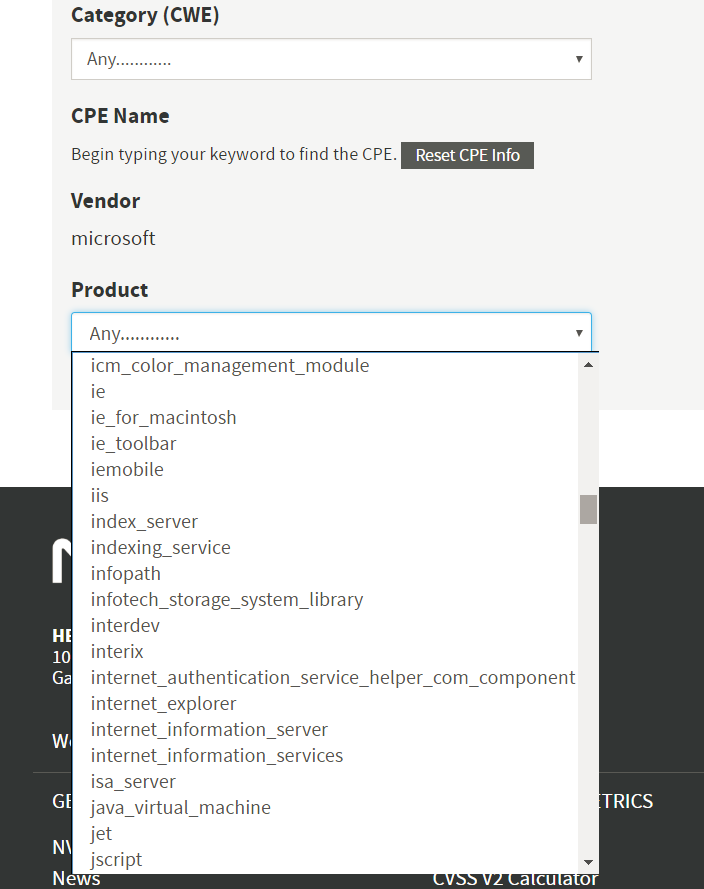
\includegraphics[width=1.0\textwidth]{image/001NVDSearchResults.png}
    \caption{Wybór filtrów w wyszukiwarce bazy danych NVD}
\end{figure}



Na rysunkach 2-5 można zauważyć iż opisy poszczególnych podatności mają podobną, jednak nie identyczną strukturę. W dwóch przypadkach, na rysunkach 2 i 3, wpis zaczyna się od określenia zakresu wpływu podatności na system, następnie podana jest nazwa producenta oraz nazwa produktu. Kolejnym elementem opisu jest wskazanie wersji produktu, w których wykryto daną podatność. W dalszej części opisu następuje wyjaśnienie istoty danej podatności. W opisach znajdujących się na rysunkach 4 oraz 5 pominięto część dotyczącą zakresu wpływu. 

\paragraph{}
Analizując poszczególne opisy można łatwo wywnioskować, że najbardziej różniącym się między poszczególnymi opisami elementem, jest określenie wersji produktu. W niektórych przypadkach opis ogranicza się do podania wersji produktu jako pojedynczej cyfry. W innych jest to doprecyzowane poprzez dopisanie po kropce dodatkowego identyfikatora wersji. Można spotkać również identyfikator wersji oznaczający pakiet, tak zwany Service Pack. W dodatku niektóre opisy zawierają mieszankę tych oznaczeń determinując poszczególne wersje z różną precyzją. Na rysunku 4 jest ukazany również przypadek, w którym podany jest zakres wersji produktu, w których można spotkać daną podatność. Wszystkie wspomniane różnice mogą powodować wysoki stopień trudności automatycznego przetwarzania opisu. Szczególnie biorąc pod uwagę fakt, że w omówionych przypadkach opisy dotyczyły tego samego produktu.

\begin{figure}[h]
    \centering
    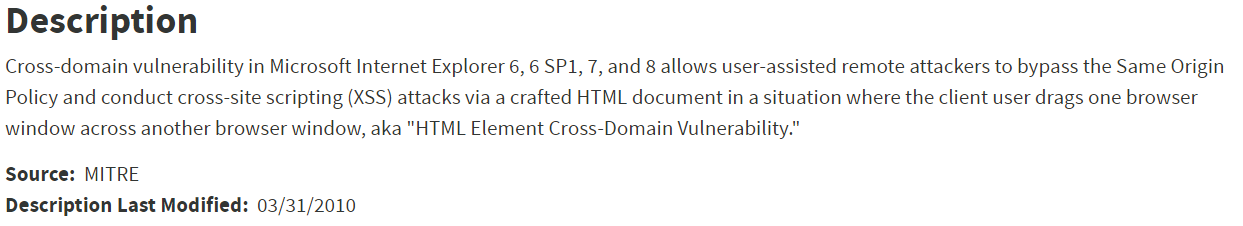
\includegraphics[width=1.0\textwidth]{image/002CVE20100494.png}
    \caption{Pole opisu wpisu CVE-2010-0494}
\end{figure}

\begin{figure}[h]
    \centering
    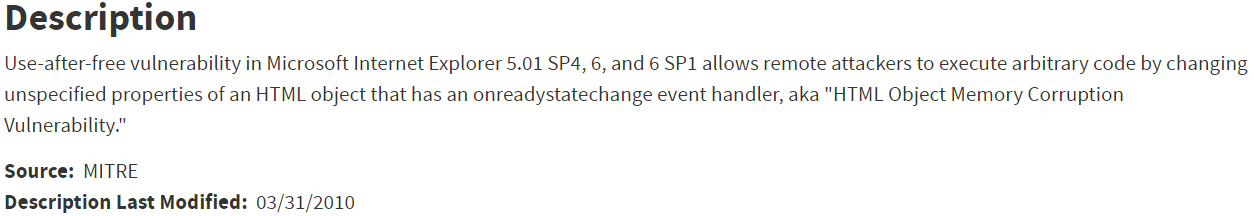
\includegraphics[width=1.0\textwidth]{image/003CVE20100491.png}
    \caption{Pole opisu wpisu CVE-2010-0491}
\end{figure}

\begin{figure}[h]
    \centering
    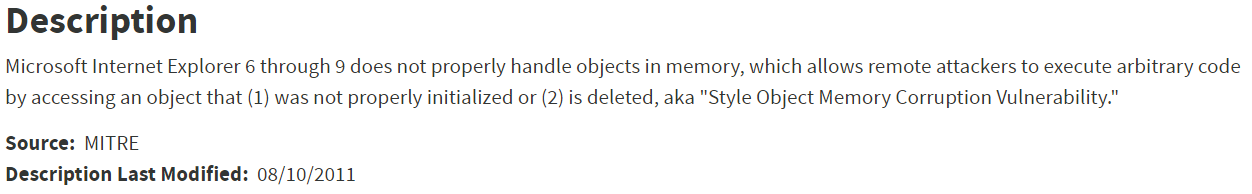
\includegraphics[width=1.0\textwidth]{image/004CVE20111964.png}
    \caption{Pole opisu wpisu CVE-2011-1964}
\end{figure}

\begin{figure}[h]
    \centering
    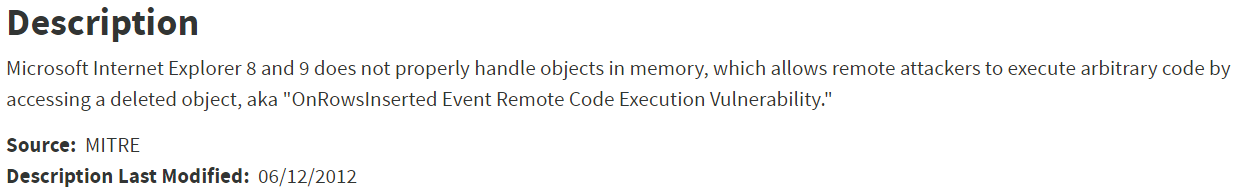
\includegraphics[width=1.0\textwidth]{image/005CVE20121881.png}
    \caption{Pole opisu wpisu CVE-2012-1881}
\end{figure}

\paragraph{}
Na zdjęciach 6-9 przedstawiono opisy dotyczące różnych produktów firmy Microsoft. Przeanalizowane zostaną pod kątem różnic w opisach wpisów CVE dotyczących aplikacji wytworzonych i rozwijanych przez tego samego producenta. 

\begin{figure}[h]
    \centering
    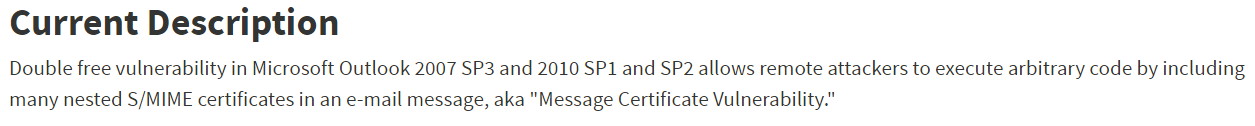
\includegraphics[width=1.0\textwidth]{image/006CVE20133870.png}
    \caption{Pole opisu wpisu CVE-2013-3870. Produkt: Microsoft Outlook}
\end{figure}

\begin{figure}[h]
    \centering
    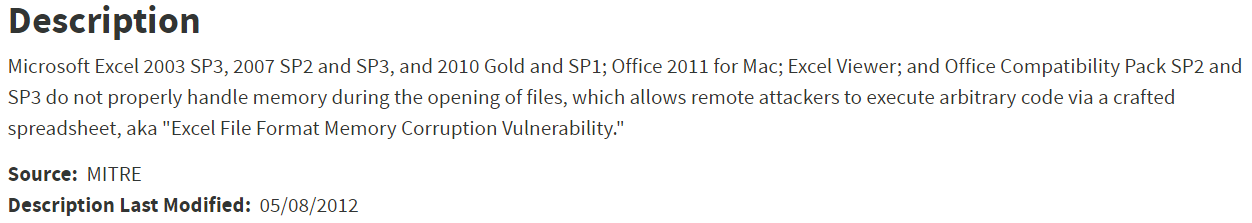
\includegraphics[width=1.0\textwidth]{image/007CVE20120141.png}
    \caption{Pole opisu wpisu CVE-2012-0141. Produkt: Microsoft Excel}
\end{figure}

\begin{figure}[h]
    \centering
    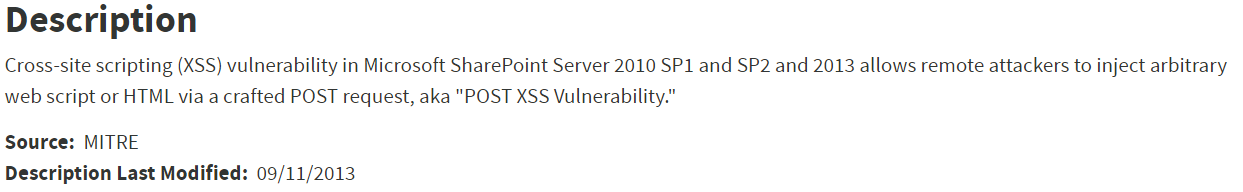
\includegraphics[width=1.0\textwidth]{image/008CVE20133180.png}
    \caption{Pole opisu wpisu CVE-2013-3180. Produkt: Microsoft SharePoint Server}
\end{figure}

\begin{figure}[h]
    \centering
    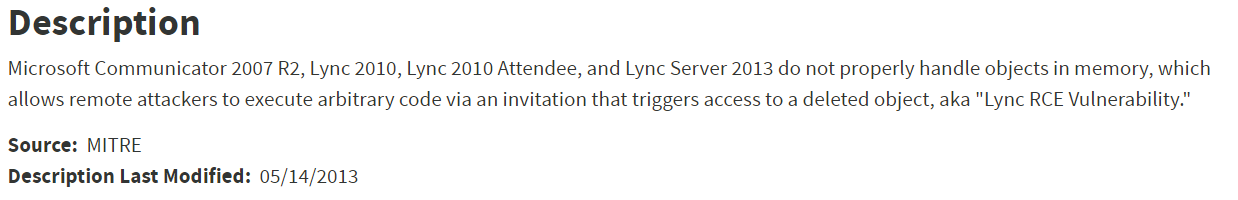
\includegraphics[width=1.0\textwidth]{image/009CVE20131302.png}
    \caption{Pole opisu wpisu CVE-2013-1302. Produkt: Microsoft Lync}
\end{figure}

\paragraph{}
Jak można zauważyć struktura opisu została zachowana jak w przypadku Microsoft Internet Explorer. To znaczy, że na początku opisu znajdują się informacje identyfikujące producenta i produkt, następnie podane są wersje produktu, w których występuje dana podatność. Zachowana została również część nazewnictwa poszczególnych wersji. Niektóre produkty mają jednak nowe identyfikatory wersji, którymi jest rok publikacji oraz występujące w opisie produktu Microsoft Excel słowo "Gold". Dodatkowym elementem opisu jest również wyszczególnienie w nim również innych produktów, w których występuje opisywana podatność. Analiza rysunków 6-9 pozwala stwierdzić, że w ramach produktów wytwarzanych przez jedną firmę istnieją różnice w nazewnictwie poszczególnych wersji, nie jest ono jednak znacząco bardziej skomplikowane, niż nazewnictwo wersji w ramach jednego produktu.

\paragraph{}
Na rysunkach 10-13 znajdują się opisy podatności występujących w produktach stworzonych przez różnych producentów. Pozwoli to przeanalizować różnice pomiędzy strukturami opisów zapewnianych przez zróżnicowane środowiska.

\begin{figure}[h]
    \centering
    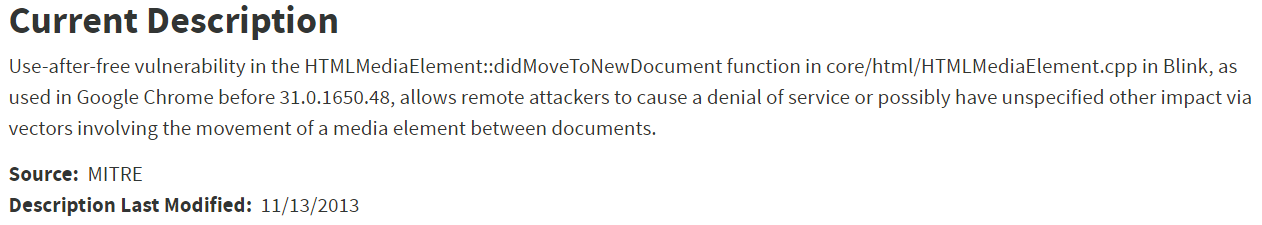
\includegraphics[width=1.0\textwidth]{image/010CVE20136622.png}
    \caption{Pole opisu wpisu CVE-2013-6622. Produkt: Google Blink}
\end{figure}

\begin{figure}[h]
    \centering
    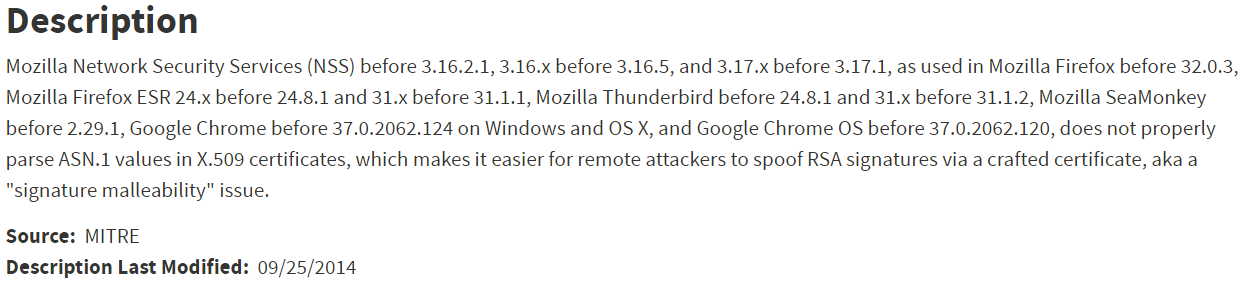
\includegraphics[width=1.0\textwidth]{image/011CVE20141568.png}
    \caption{Pole opisu wpisu CVE-2014-1568. Produkt: Mozilla Network Security Services}
\end{figure}

\begin{figure}[h]
    \centering
    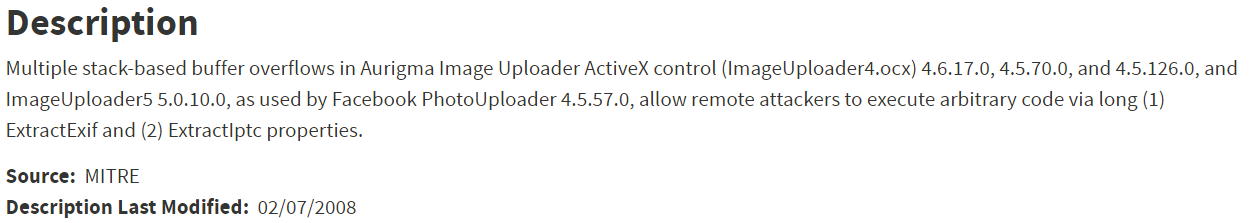
\includegraphics[width=1.0\textwidth]{image/012CVE20080660.png}
    \caption{Pole opisu wpisu CVE-2008-0660. Produkt: Aurigma Image Uploader ActiveX}
\end{figure}

\begin{figure}[h]
    \centering
    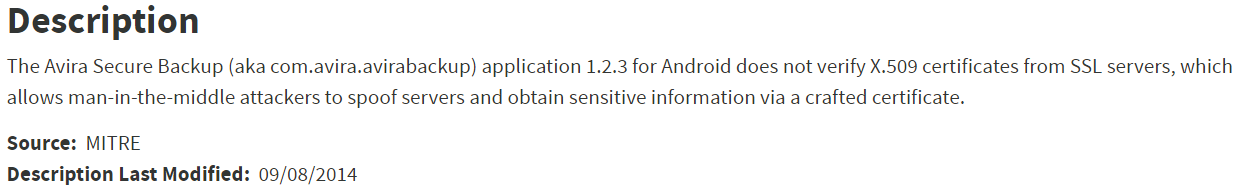
\includegraphics[width=1.0\textwidth]{image/013CVE20145576.png}
    \caption{Pole opisu wpisu CVE-2014-5576. Produkt: Avira Secure Backup}
\end{figure}







\newpage
%% =========================== BIBLIOGRAFIA ==============================
\section*{ }
\addcontentsline{toc}{section}{Bibliografia}
\markboth{Bibliografia}{}
\bibliographystyle{plain}
\renewcommand{\refname}{Bibliografia}
\begin{thebibliography}{}


\bibitem{mitre_cve_basics}
https://cve.mitre.org/about/faqs.html

\bibitem{cve_mitre_terms}
https://cve.mitre.org/about/terminology.html

\bibitem{cve_mitre_cna_doc}
"CVE Overview for Prospective CNAs", Mitre Corporation, Version 1.0, 29 Wrzesień 2018
%% https://cve.mitre.org/cve/cna/CVE_Overview_for_Prospective_CNAs_v1.0.pdf

\bibitem{nvd_official}
https://nvd.nist.gov
  

\end{thebibliography}

\newpage
%% =========================== SPIS ILUSTRACJI ===========================
%%\section*{ }
%%\listoffigures
%%\newpage
%%\addcontentsline{toc}{section}{Spis rysunków}

%%\newpage
%% =========================== SPIS TABEL ===========================
%%\section*{ }
%%\listoftables
%%\newpage
%%\addcontentsline{toc}{section}{Spis tabel}

%%\newpage
%% =========================== SPIS LISTINGÓW ===========================
%%\section*{ }
%%\renewcommand{\lstlistlistingname}{Spis listingów}
%%\lstlistoflistings 
%%\newpage
%%\addcontentsline{toc}{section}{Spis listingów}



%%\newpage
%% =========================== DODATKI ===========================
%%\section*{Dodatki}
%%\addcontentsline{toc}{section}{Dodatki}
%%\markboth{Dodatki}{}
%%\paragraph{}

\end{document}